% Staircase paper for 18.821 Fall 2012 project 3.
% Authors: Daniel Grazian, Michael Mekonnen, Agustin O Venezuela III

\documentclass[12pt]{amsart}

% Keep everything here in alphabetical order, please! :) -jven

% Packages

\usepackage{amssymb}
\usepackage{graphicx}

% Enumeration

\newtheorem{theorem}{Theorem}[section]

\newtheorem{conjecture}[theorem]{Conjecture}
\newtheorem{corollary}[theorem]{Corollary}
\newtheorem{definition}[theorem]{Definition}
\newtheorem{example}[theorem]{Example}
\newtheorem{examples}[theorem]{Examples}
\newtheorem{lemma}[theorem]{Lemma}
\newtheorem{proposition}[theorem]{Proposition}
\newtheorem{remarks}[theorem]{Remarks}
\newtheorem{remark}[theorem]{Remark}

% Utility commands
% Inverse factorial
\newcommand{\ifact}{\mu}
% Determinant of our special matrix
\newcommand{\M}{M}
% Determinant of our special matrix with a row changed
\newcommand{\N}{N}
% Real numbers
\newcommand{\R}{\mathbb{R}}
% Figures: \newfigure{label}{caption}{content}
\newcommand{\newfigure}[3]{
\begin{figure}
#3
\caption{#2 \label{#1}}
\end{figure}
}
% Sections: \newsection{title}{label}
\newcommand{\newsection}[2]{
\section{#1 \label{#2}}
}

\title{A Staircase Model of Erosion}
\author{Daniel Grazian, Michael Mekonnen, Agustin O Venezuela III}
\date{December 3, 2012}

\begin{document}

\begin{abstract}
TODO(dgrazian, jven, mikemeko)
\end{abstract}

\maketitle

\newsection{Introduction}{sec:intro}
In this paper, we consider the random process of forming staircases by dropping blocks into an infinite row of infinitely tall columns.

More concretely, consider partitioning the first quadrant of $\R^2$ into axis-aligned columns of width $1$, as in Figure $\ref{fig:columns}$. We will index the columns starting at $0$.

\newfigure{fig:columns}{Partitioning of the first quadrant into columns}{
TODO
}

Now consider iteratively placing unit squares (blocks) into these columns. We will say that a block is at location $(i, j)$ for non-negative integers $i, j$ if it is axis-aligned and its bottom-left vertex is at $(i, j)$. At each step, a block can be placed at $(i, j)$ if and only if (1) $i = 0$ or there is a block at $(i - 1, j)$ and (2) $j = 0$ or there is a block at $(i, j - 1)$. Figure $\ref{fig:dropblocks}$ shows an example of a valid sequence of placing $5$ blocks. We will usually refer to such a sequence of placements a \textit{dropping of $5$ blocks}, for obvious reasons. We call a configuration of $n$ blocks in the first quadrant a \textit{staircase} if it can be obtained by dropping $n$ blocks.

\newfigure{fig:dropblocks}{Example of dropping $5$ blocks}{
TODO
}

We will refer to a staircase as the monotonically decreasing finite sequence of positive integers $(b_i)$, where $b_i$ is the number of blocks in column $i$. For example, the last staircase in Figure \ref{fig:dropblocks} can be written as $(hi,hi,hi,hi,hi)$. Note that we do not include columns that do not contain any blocks.

We are interested in constructing random staircases: beginning with no blocks, we consider all the locations $(i, j)$ at which a block can be validly placed, choose such a location uniformly at random, and place a block there. This raises various interesting questions regarding the distribution over the shape of the resulting staircase when $n$ blocks are dropped.

TODO(mikemeko, jven): change this
To begin, Section \ref{sec:numstaircases} will address the question of how many staircases exist with $n$ blocks. Section \ref{sec:expectedcolumns} will present numerical results for the expected number of columns for a staircase with $n$ blocks. Finally, Section \ref{sec:twocolumn} will present exact results for the variant of the problem in which we restrict staircases to having at most $2$ columns.

\newsection{Number of Staircases with $n$ Blocks}{sec:numstaircases}
Our investigation into the distribution over staircase shapes begins with determining how many staircase shapes exist using $n$ blocks.

\begin{theorem}
The number of staircases with $n$ blocks is equal to the number of partitions of $n$ (the number of ways to write $n$ as a sum of positive integers, irrespective of the order of the parts).
\begin{proof}
There is an obvious bijection $f$ between staircase with $n$ blocks and partitions of $n$. We map the staircase $(b_i)$ with $n$ blocks to the partition $n=\sum b_i$.

$f$ is injective. If $(b_i)\neq (b_i')$ are two distinct staircases, then $n = \sum b_i = \sum b_i'$ are two partitions of $n$ such that with the parts written in monotonically decreasing order, we have some $b_i\neq b_i'$. It follows that the two partitions are distinct.

$f$ is also surjective. Given a partition $n = \sum a_i$, we can sort $(a_i)$ in monotonically decreasing order, yielding $(b_i)$. $f$ clearly maps $(b_i)$ to the partition $\sum a_i$.

The result follows.
\end{proof}
\end{theorem}

For increasing $n$ beginning with $n = 0$, the numbers of partitions of $n$ are $1, 1, 2, 3, 5, 7, 11, \ldots$. Unfortunately, this sequence is known to grow exponentially with $n$: for $n = 100$, there are $190,569,292$ partitions. This appears to make our original goal of finding a distribution over staircase shapes difficult as there are exponentially many objects to which a probability is to be assigned. For this reason, we instead consider the distribution over the number of columns in the next section, the number of which is clearly linear in $n$.

\newsection{Number of ways to construct a staircase}{sec:numconstructions}
Let us now focus on the number of ways to construct a particular staircase $(c_0, c_1, \dots, c_k)$. For instance, there are $2$ ways to construct the $(2,1)$ staircase. We begin with a few formalizing definitions, and then we proceed to developing a closed form expression for the quantity we are studying.

\begin{definition}
Let $T(c_0, c_1, \dots, c_k)$ denote the number of ways to construct the $(c_0, c_1, \dots, c_k)$ staircase, where we assume that $c_0 \geq c_1 \geq \dots \geq c_k > 0$.
\end{definition}

\begin{definition}
For any integer $i$, we define
$$
\ifact(i) = 
\begin{cases}
\frac{1}{i!} & \text{if } i \geq 0 \\
0 & \text{otherwise.}
\end{cases}
$$
\end{definition}

To motivate the definition of $\ifact$, consider the quantity $\binom{1}{-1}$. Intuitively, this quantity should be $0$ since there are $0$ ways to choose $-1$ items from a set containing $1$ item. By definition, we have that $\binom{1}{-1} = \frac{1}{(-1)!2!}$. Thus, $\frac{1}{(-1)!} = \ifact(-1)$ ought to be $0$.

\begin{definition}
For a sequence of integers $c_0, c_1, \dots, c_k$ such that $c_0 \geq c_1 \geq \dots \geq c_k \geq 0$, we define
$$
\M(c_0, c_1, \dots, c_k) = \left|
\begin{matrix}
\ifact(c_0) & \ifact(c_0+1) & \cdots & \ifact(c_0+k) \\
\ifact(c_1-1) & \ifact(c_1) & \cdots & \ifact(c_1+k-1) \\
\vdots & \vdots & \ddots & \vdots \\
\ifact(c_k-k+1) & \ifact(c_k-k+2) & \cdots & \ifact(c_k) \\
\end{matrix} \right|
$$
\end{definition}

\begin{definition}
For a sequence of integers $c_0, c_1, \dots, c_k$ such that $c_0 \geq c_1 \geq \dots \geq c_k \geq 0$, we define
$$
\N_i(c_0, c_1, \dots, c_k) = \left|
\begin{matrix}
\ifact(c_0) & \ifact(c_0+1) & \cdots & \ifact(c_0+k) \\
\vdots & \vdots & \ddots & \vdots \\
-i\ifact(c_i-i) & (1-i)\ifact(c_i - i + 1) & \cdots & (k-i) \ifact(c_i+k-i) \\
\vdots & \vdots & \ddots & \vdots \\
\ifact(c_k-k) & \ifact(c_k-k+2) & \cdots & \ifact(c_k) \\
\end{matrix} \right|
$$
\end{definition}

Let us now write a recurrence relation for $T(c_0, c_1, \dots, c_k)$.
\begin{lemma}
\begin{align*}
T(c_0, c_1, \dots, c_k) = & T(c_0-1, c_1, \dots, c_k) + \\
&  T(c_0, c_1-1, \dots, c_k) + \\
& \dots \\
& T(c_0, c_1, \dots, c_k-1)
\end{align*}
\label{lem:recurrence}
\end{lemma}

\begin{proof}
TODO(mikemeko): there are special conditions here, mention them?

The $(c_0, c_1, \dots, c_k)$ staircase can be built in one of $k$ different ways: build the $(c_0-1, c_1, \dots, c_k)$ staircase and then add a block to the $0^{th}$ column, or build the $(c_0, c_1-1, \dots, c_k)$ staircase and then add a block to the $1^{st}$ column, etc. The recurrence captures exactly this idea.
\end{proof}

Now we proceed to our main result.

\begin{theorem}
$$
T(c_0, c_1, \dots, c_k) = (c_0 + c_1 + \dots + c_k)! \M(c_0, c_1, \dots, c_k)
$$
\end{theorem}

\begin{proof}
We prove this by induction on $c_0, c_1, \dots, c_k$.

TODO(mikemeko): is this base case good? say more about how we can compute any $T(c_0, c_1, \dots, c_k)$ starting with these.

In the base case, we look at all cases in which $c_i \geq 0 \forall i = 0,1,\dots,k$ and $\sum_{i=0}^{k}{c_i} = 1$. First, we have that
$$
T(1,0,\dots,0) = \M(1,0,\dots,0)=\left|
\begin{matrix}
1 & \ifact(2) & \ifact(3) & \cdots & \ifact(k) \\
0 & 1 & \ifact(2) & \cdots & \ifact(k-2) \\
0 & 0 & 1 & \cdots & \ifact(k-3) \\
\vdots & \vdots & \vdots & \ddots & \vdots \\
0 & 0 & 0 & \cdots & 1 \\
\end{matrix} \right| = 1,
$$
as desired. We get the last equality by observing that the determinant is of an upper-triangular matrix wish diagonal terms that are all $1$. Next, consider setting $c_i = 1, i > 0$ and all other columns $0$. In this case, the $(i-1)^{st}$ and $i^{th}$ rows in the matrix become identical, and, therefore, the determinant equals $0$, as desired.

In the inductive step, we assume that the theorem holds for $T(c_0-1,c_1,...,c_n)$, $T(c_0,c_1-1,...,c_n)$, $\dots$, $T(c_0,c_1,...,c_n-1)$, and show that it also holds for $T(c_0,c_1,...,c_n)$. Here we use the recurrence in Lemma \ref{lem:recurrence}.

\begin{align*}
T(c_0, \dots, c_k) = & T(c_0-1, \dots, c_k) + \dots + T(c_0, \dots, c_k-1) \\
= & (c_0 + \dots + c_k-1)! \\
& ( \M(c_0-1, \dots, c_k) + \dots + \M(c_0, \dots, c_k-1)) \\
= & (c_0 + \dots + c_k-1)! \\
& ( c_0 \M(c_0, \dots, c_k) + \N_0(c_0, c_1, \dots, c_k) + \\
& c_1 \M(c_0, \dots, c_k) + \N_1(c_0, c_1, \dots, c_k) + \\
& \dots + \\
& c_k \M(c_0, \dots, c_k) + \N_k(c_0, c_1, \dots, c_k) ) \\
= & (c_0 + \dots + c_k)! \M(c_0,\dots,c_k) + \\
& (c_0+\dots+c_k-1)! (\N_0(c_0,\dots,c_k) + \dots + \N_k(c_0,\dots,c_k)).
\end{align*}

TODO(mikemeko) elaborate.

Thus, all that remains to show now is that
$$
\N_0(c_0,\dots,c_k) + \dots + \N_k(c_0,\dots,c_k) = 0.
$$
Each of the terms in the sum is a determinant of a $(k+1)\times(k+1)$ matrix, which is a linear combination of $(k+1)!$ terms. Note that each of these terms is the same across the $k+1$ determinants, the only difference being in the leading constant coefficients. Let us look at the $k+1$ constant coefficients accompanying a particular term. Let us denote this term by $(\sigma_0, \sigma_1, \dots, \sigma_k)$, a permutation of $(0, 1, \dots, k)$, with $\sigma_i$ indicating the column number of the term from the $i^{th}$ row. Note that the constant coefficient for this term from the determinant $\N_i(c_0,\dots,c_k)$ is $\sigma_i - i$. This follows directly from the structure of $\N_i(c_0,\dots,c_k)$. Now, we can add up all the contributions from the $k+1$ determinants to get the final constant coefficient for the factor:
$$
\sum_{i=0}^{k}{\sigma_i-i} = 0.
$$
Thus, we have that each factor contributes nothing to the sum of determinants, giving us the result we need.

\end{proof}

\newsection{Expected Number of Columns}{sec:expectedcolumns}
We now consider the number of columns that occur when $n$ blocks are dropped. Our results at this point are rather minimal, but we present what we have.

There is a $\frac{1}{2^{n-1}}$ probability of a randomly constructed $n$-block staircase having one column. The only staircase of $n$ blocks with 1 column is $(n)$, a tower of $n$ blocks. The first block is guaranteed to be dropped in the first column. For $1<k \leq n$, the $k^{th}$ block is added to a staircase consisting of $(k-1)$ blocks in a single column. The $k^{th}$ block therefore has probability $\frac{1}{2}$ of being dropped in the first cloumn. So the probability of obtaining the $n$-block staircase $(n)$ is $\frac{1}{2^n}$.

Similarly, the probability of obtaining a staircase with $n$ columns is $\frac{1}{2^{n}}$. The only $n$-block staircase with $n$ columns is $(1, 1, \ldots, 1)$, and the probability of obtaining this staircase is $\frac{1}{2^{n}}$ by reasoning similar to that in the paragraph above.

However, the probability distribution of the number of columns in a randomly constructed $n$-block staircase is not symmetric. For example, for $n > 4$ it is more likely for a randomly constructed $n$-block staircase to contain $2$ columns than to contain $n-1$ columns. The only staircase with $n-1$ columns is $(2, 1, 1, \ldots, 1)$. There are $n-1$ block-dropping sequences that form this staircase, because any block after the $1^{st}$ can be the $2^{nd}$ block dropped in the $1^{st}$ column. Each of these seqences has probability less than $\frac{1}{2^{n-1}}$ of ocurring, so the probability of an $n$-block staircase having $n-1$ columns is less than $\frac{n}{2^{n-1}}$.  In contrast, there are $\lfloor \frac{n}{2} \rfloor$ staircases with $2$ columns. These are $(n-1, 1), (n-2, 2), \ldots, (\lceil \frac{n}{2} \rceil, \lfloor \frac{n}{2} \rfloor)$. The first of these staircases alone has the same probability of occurring  as the one staircase with $n-1$ columns. So the probability of a $n-1$ column staircase must be greater than that of a $2$-column staircase.

In general we suspect that the probability distribution of the number of columns in a randomly constructed staircase is skewed left. Specifically, for $1 < k < \frac{n}{2}$, the probability of a staircase having $k$ columns is greater than the probability of it having $n-k+1$ columns. For example, see figure $\ref{fig:prob_distribution}$ for the probability distribution with 10 blocks. (TODO : proof?)

We also obtain a lower bound on the expectation of the number of columns in a randomly generated staircase.

\begin{theorem}
\label{lower_bound}
The expected number of blocks required for a staircase to reach $n$ columns is less than or equal to $\displaystyle\sum_{i=1}^{n}i = \frac{n(n+1)}{2}$
\end{theorem}

\begin{proof}
Consider the construction of a staircase $1$ block at a time. Given a staircase with $k-1$ columns the probability that the next block will create an extra column is greater than or equal to $\frac{1}{k}$, so the expected number of blocks required to create the next column is less than or equal to $k$. Therefore, the number of blocks required to get to the $n^{th}$ column is less than or equal to $1 + 2 + \ldots + n$. The theorem follows.
\label{thm:lower_bound}
\end{proof}

Theorem \ref{thm:lower_bound} implies that the expected number of columns in a randomly generated staircase of $\frac{n(n+1)}{2}$ blocks is greater than or equal to $n$. This means that the expected number of columns in a staircase of $n$ blocks grows at least on the order of $\sqrt{n}$.





\begin{figure}
\caption{Probability Distribution of Number of Columns in Staircase With Ten Blocks}
\label{fig:prob_distribution}
\begin{center}
\begin{tabular}{| c | c |}
\hline
Number of Columns & Probability\\ \hline
1 & .0020\\ \hline
2 & .0582\\ \hline
3 & .2099\\ \hline
4 & .2910\\ \hline
5 & .2254\\ \hline
6 & .1294\\ \hline
7 & .0557\\ \hline
8 & .0208\\ \hline
9 & .0057\\ \hline
10 & .0020\\ \hline
\end{tabular}
\end{center}
\end{figure}
  





TODO More in this section?

\newsection{2-Column Staircases}{sec:twocolumn}
Now we restrict ourselves to staircases of the form $(m,n)$ that have at most $2$ columns. We are interested in finding the number of ways to construct the $(m,n)$ staircase.

\begin{definition}
Let $T(m,n)$ denote the number of different ways to construct the $(m,n)$ staircase.
\end{definition}

We start by writing a recurrence to describe $T(m,n)$:
\begin{equation}
T(m,n) = \left\{ 
  \begin{array}{l l}
    T(m-1,n) + T(m,n-1) & \quad \text{if $m \geq n > 0$}\\
    1 & \quad \text{if $m \geq n = 0$}\\
    0 & \quad \text{otherwise}\\
  \end{array} \right.
\label{eqn:2-recurrence}
\end{equation}
The idea behind this recurrence is that, in the case where $m > n$, we can construct the $(m,n)$ staircase by first constructing the $(m-1,n)$ staircase and then adding a block to the first column or by constructing the $(m,n-1)$ staircase and then adding a block to the second column. There is exactly $1$ way to construct the $(m,0)$ staircase, and that is by adding a block to the first column $m$ times. Finally, if $m < n$, it is not possible to construct such a staircase by definition.

Instead of attempting to solve this recurrence algebraically, we will come up with an answer through a combinatorial argument, and use the recurrence to verify that the answer is correct.

Since the interesting case in the recurrence is the $m \geq n > 0$ case, we will focus on that condition in the analysis that follows. The other cases are simply base cases for the recurrence. Note that in our setting, constructing the $(m,n)$ staircase requires that the second column be no higher than the first column throughout the construction. Since we have $m+n$ blocks to work with, it is clear that there are generally $\binom{m+n}{m}$ ways to produce the $(m,n)$ staircase (corresponding to the $m$ blocks out of the $m+n$ that we choose to put in the first column), but some of these violate the staircase construction condition. So now we need to find the number of of ways to to produce the $(m,n)$ staircase using $m+n$ blocks such that, at some point during the construction, the second column is higher than the first one. We will find this number using a combinatorial argument.

We can think about constructing the $(m,n)$ staircase as going form $(0,0)$ to $(m,n)$ on the $2$-dimensional lattice by taking unit steps to the right or up. The staircase construction condition requires that this path never cross the diagonal line in the lattice. So our task now is to count the number of paths that do cross the diagonal. We shall do this using the reflection principle: we will create a bijection between the set of paths from $(0,0)$ to $(m,n)$ that do cross diagonal to the set of all paths from $(0,0)$ to $(n-1,m+1)$.

Given a path from $(0,0)$ to $(m,n)$ that crosses the diagonal, we can construct the corresponding path from $(0,0)$ to $(n-1,m+1)$ as follows. Let us denote the first time the original path crosses the diagonal by the point $(i,i+1)$ for some integer $i < n$. Now we can define the corresponding path from $(0,0)$ to $(n-1,m+1)$ to be exactly the same as the original path up until $(i,i+1)$, but the reflection of the original path after $(i,i+1)$. That is, where the original path takes a unit step to the right, the new path takes a unit step up, and vice versa. To verify that the end point of the new path is $(n-1,m+1)$, note that the original path is left with a total of $m-i$ steps to the right, which means that the new path is left with a total of $m-i$ steps up. Similarly the original path is left with a total of $n-i-1$ steps up, which means the new path is left with a total of $n-i-1$ steps to the right. So the final point of the new path is given by $(i+(n-i-1), i+1+(m-i)) = (n-1,m+1)$, as claimed.

Given a path from $(0,0)$ to $(n-1,m+1)$, we can construct the corresponding path from $(0,0)$ to $(m,n)$ that crosses the diagonal using the same procedure explained above. Note that the original path must have a point $(i,i+1)$ since $m+1>n-1$. We can verify that the new path has end point $(m,n)$ using a similar analysis: $(i+(m+1-i-1),i+1+(n-1-i)) = (m,n)$, as desired.

\begin{figure}
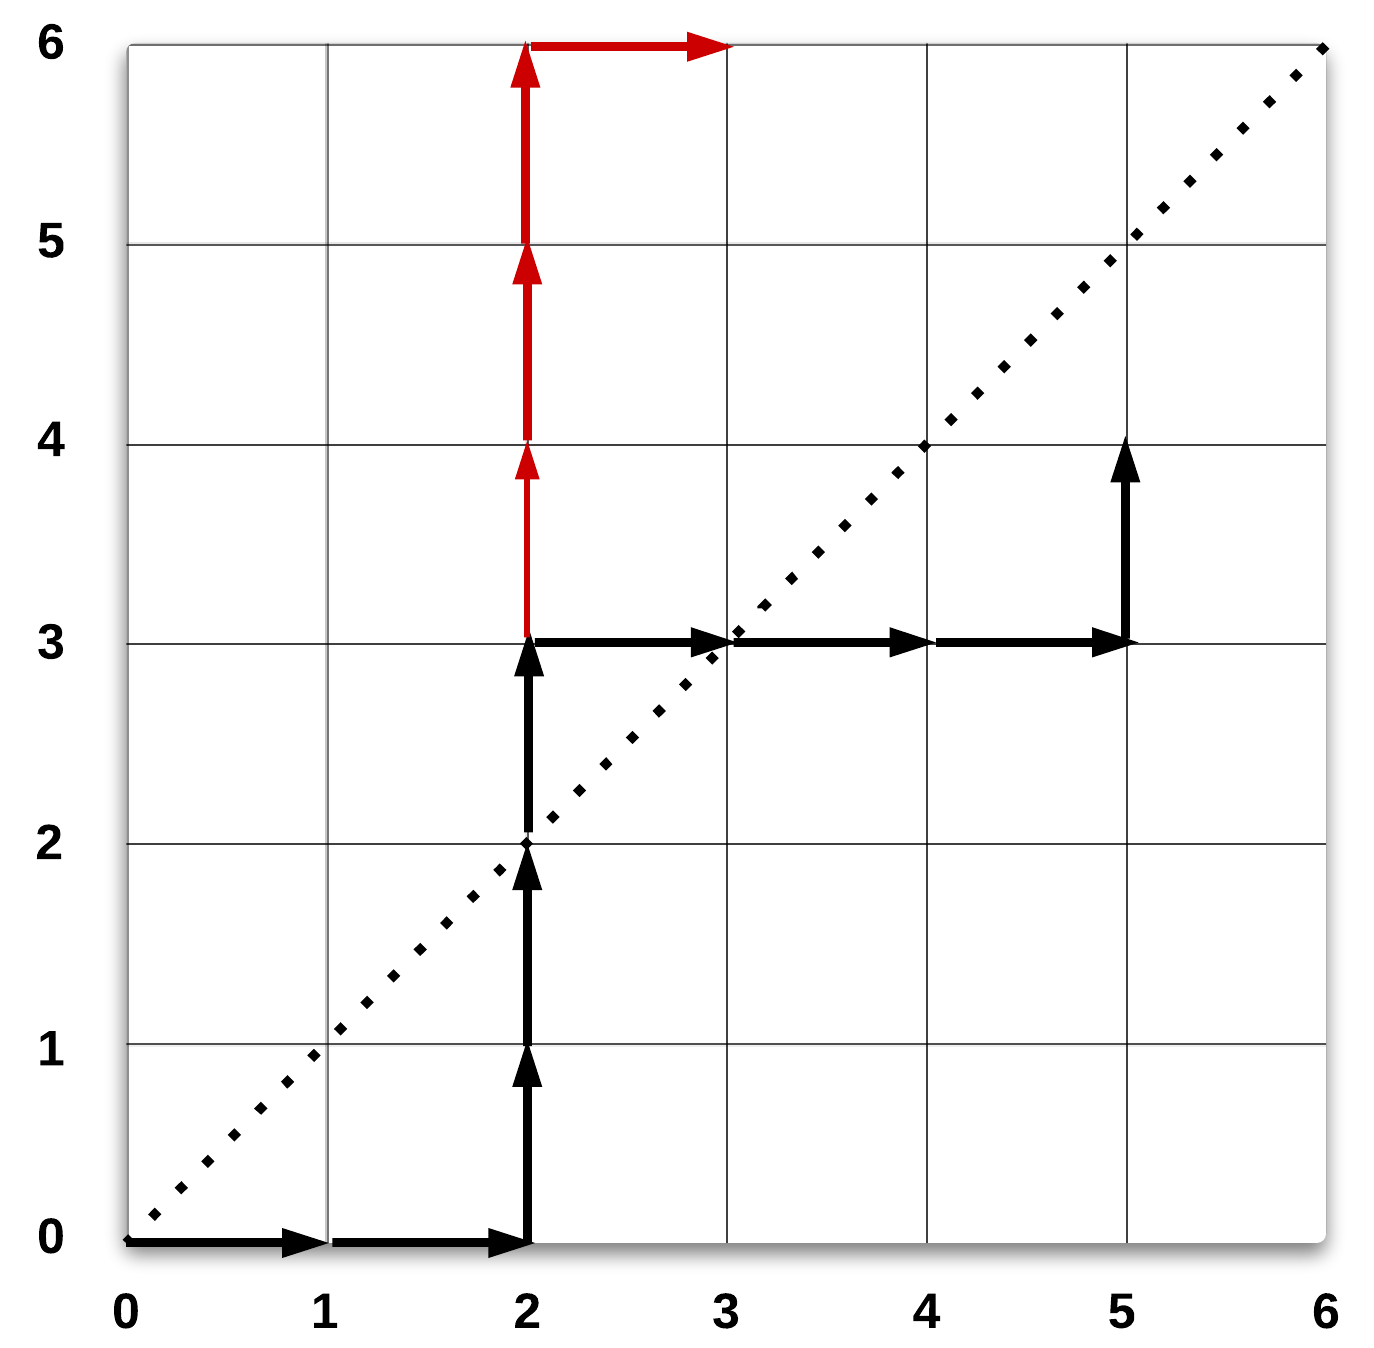
\includegraphics[width=10cm]{reflection.png}
\caption{A path from $(0,0)$ to $(m=5, n=4)$ that crosses the diagonal, and its corresponding path from $(0,0)$ to $(n-1=3, m+1=6)$, shown in red.}
\label{fig:reflection}
\end{figure}

We have thus established the desired bijection. An example pair is given in Figure \ref{fig:reflection} where $m=5$ and $n=4$. This bijection leads to the conclusion that the number of constructions of the $(m,n)$ staircase for which, at some point during the construction, the second column is higher than the first column is $\binom{m+n}{n-1}$. Thus, we have the following expression for $T(m,n)$.

\begin{theorem}
$T(m,n) = \binom{m+n}{m} - \binom{m+n}{n-1}, \text{if $m \geq n > 0$.}$
\end{theorem}

\begin{proof}
We prove this by induction on $m$ and $n$.

In the base case, it suffices to have that $T(0,0) = T(1,0) = 1$, and these equalities follow from the standard definition of the binomial coefficients:
$$
\binom{k}{l} =
\begin{cases}
\frac{k!}{l!(k-l)!} & \text{if } 0 \leq l \leq k \\
0 & \text{otherwise.}
\end{cases}
$$

In the inductive step, we consider two cases. First, the case where $m=n>0$. Here, we have, by definition, that $T(m-1,n)=0$. We assume that the equality holds for $T(m,n-1)$, and we get

\begin{align*}
T(m,n) & = T(m,n-1) \\
& = T(n,n-1) \\
& = \binom{2n-1}{n} - \binom{2n-1}{n-2} \\
& = \Bigg(\binom{2n-1}{n} + \binom{2n-1}{n-1}\Bigg)-\Bigg(\binom{2n-1}{n-1} + \binom{2n-1}{n-2}\Bigg) \\
& = \binom{2n}{n} - \binom{2n}{n-1} \\
& = \binom{m+n}{m} - \binom{m+n}{n-1},
\end{align*}
as desired. The previous to last equality follows from Pascal's identity.

Next, for the case where $m>n>0$, we assume that the equality holds for $T(m-1,n)$ and $T(m,n-1)$ and we get
\begin{align*}
T(m,n) & = T(m-1,n) + T(m,n-1) \\
& = \binom{m+n-1}{m-1} - \binom{m+n-1}{n-1} + \binom{m+n-1}{m} - \binom{m+n-1}{n-2} \\
& = \Bigg(\binom{m+n-1}{m-1} + \binom{m+n-1}{m}\Bigg) - \Bigg(\binom{m+n-1}{n-1} + \binom{m+n-1}{n-2}\Bigg) \\
& = \binom{m+n}{m} - \binom{m+n}{n-1},
\end{align*}
as desired. Once again, the last equality follows from Pascal's identity.
\end{proof}

An interesting result we obtain is that $T(n,n) = \binom{2n}{n} - \binom{2n}{n-1}$ is exactly the $n^{th}$ Catalan number. In the $2$x$n$ rectangular $(n,n)$ staircase, we can think about the blocks in the first column as left parentheses ``(" and the blocks in the second column as right parentheses ``)". Since the staircase construction condition produces a correct parenthesization, this leads to a familiar interpretation of the Catalan numbers. 

\end{document}